\subsection{Event Selection} \label{sec:WBoson_Analysis_Selection}


This section describes the set of criteria defined to select the events in this analysis. The signal events, determined by the process \WToMuNu, are characterised by a high \pt muon and the presence of MET, originated from the undetected neutrino. Moreover, events with similar characteristics can also be produced by other background processes, such as QCD multi-jet events (QCD background), Drell-Yan (DY) dilepton events or Electro-Weak (EWK) decays, which are further described in \sect{sec:WBoson_Analysis_BackgroundSources}.


\subsubsection{Global Event Filter} \label{sec:WBoson_Analysis_EventFilter}


The \pPb standard event selection criteria recommended by the HIN Global Observable (GO) group are applied in order to ensure that the events are not contaminated by non-collision events \cite{Centrality_pPb}. The different selections included in the \pPb Global Event Filter (GEF) are described below:

\begin{itemize}
\item Primary Vertex filter: Requires a primary vertex reconstructed from at least two tracks, within $\left|v_{z}\right| < 25$~\cm and $\rho < 2$~\cm, of the nominal interaction point.
\item HF Coincidence filter: Requires at least one tower on each side of the interaction point in the HF calorimeter with an energy deposit per tower of at least 3~\GeV.
\item Beam-Scraping filter: Requires at least 25$\%$ of all the tracks in the event to pass the high purity quality conditions.
\end{itemize}

The impact of the GEF was checked both in data and MC. Only 0.08~$\%$ of events in data and 0.06~$\%$ of events in MC, passing all the analysis cuts summarized in \sect{sec:WBoson_Analysis_WSelection}, were removed by the filters.

\subsubsection{Drell-Yan Veto} \label{sec:WBoson_Analysis_DrellYanVeto}

A Drell-Yan veto is applied to suppress the contribution from \DYToMuMu background events. This veto removes events that contain at least two opposite sign muons with $\pt > 15$~\GeVc passing the Tight muon ID and the relative muon isolation cut $iso < 0.15$, defined in \sect{sec:WBoson_Analysis_MuonIdentification} and \sect{sec:WBoson_Analysis_MuonIsolation}, respectively .

The probability that Drell-Yan events survive the veto is checked using the official Drell-Yan MC samples mentioned in \tab{tab:MCSamples}. The denominator of the Drell-Yan Veto effiency is  filled with the muons passing all the \W analysis cuts (see \sect{sec:WBoson_Analysis_WSelection}), while the numerator is filled with the same muons as long as the event pass the Drell-Yan veto. The MC survival probability is shown in \fig{fig:DrellYanVetoZEfficiency2D}.

\begin{figure}[htb]
 \begin{center}
   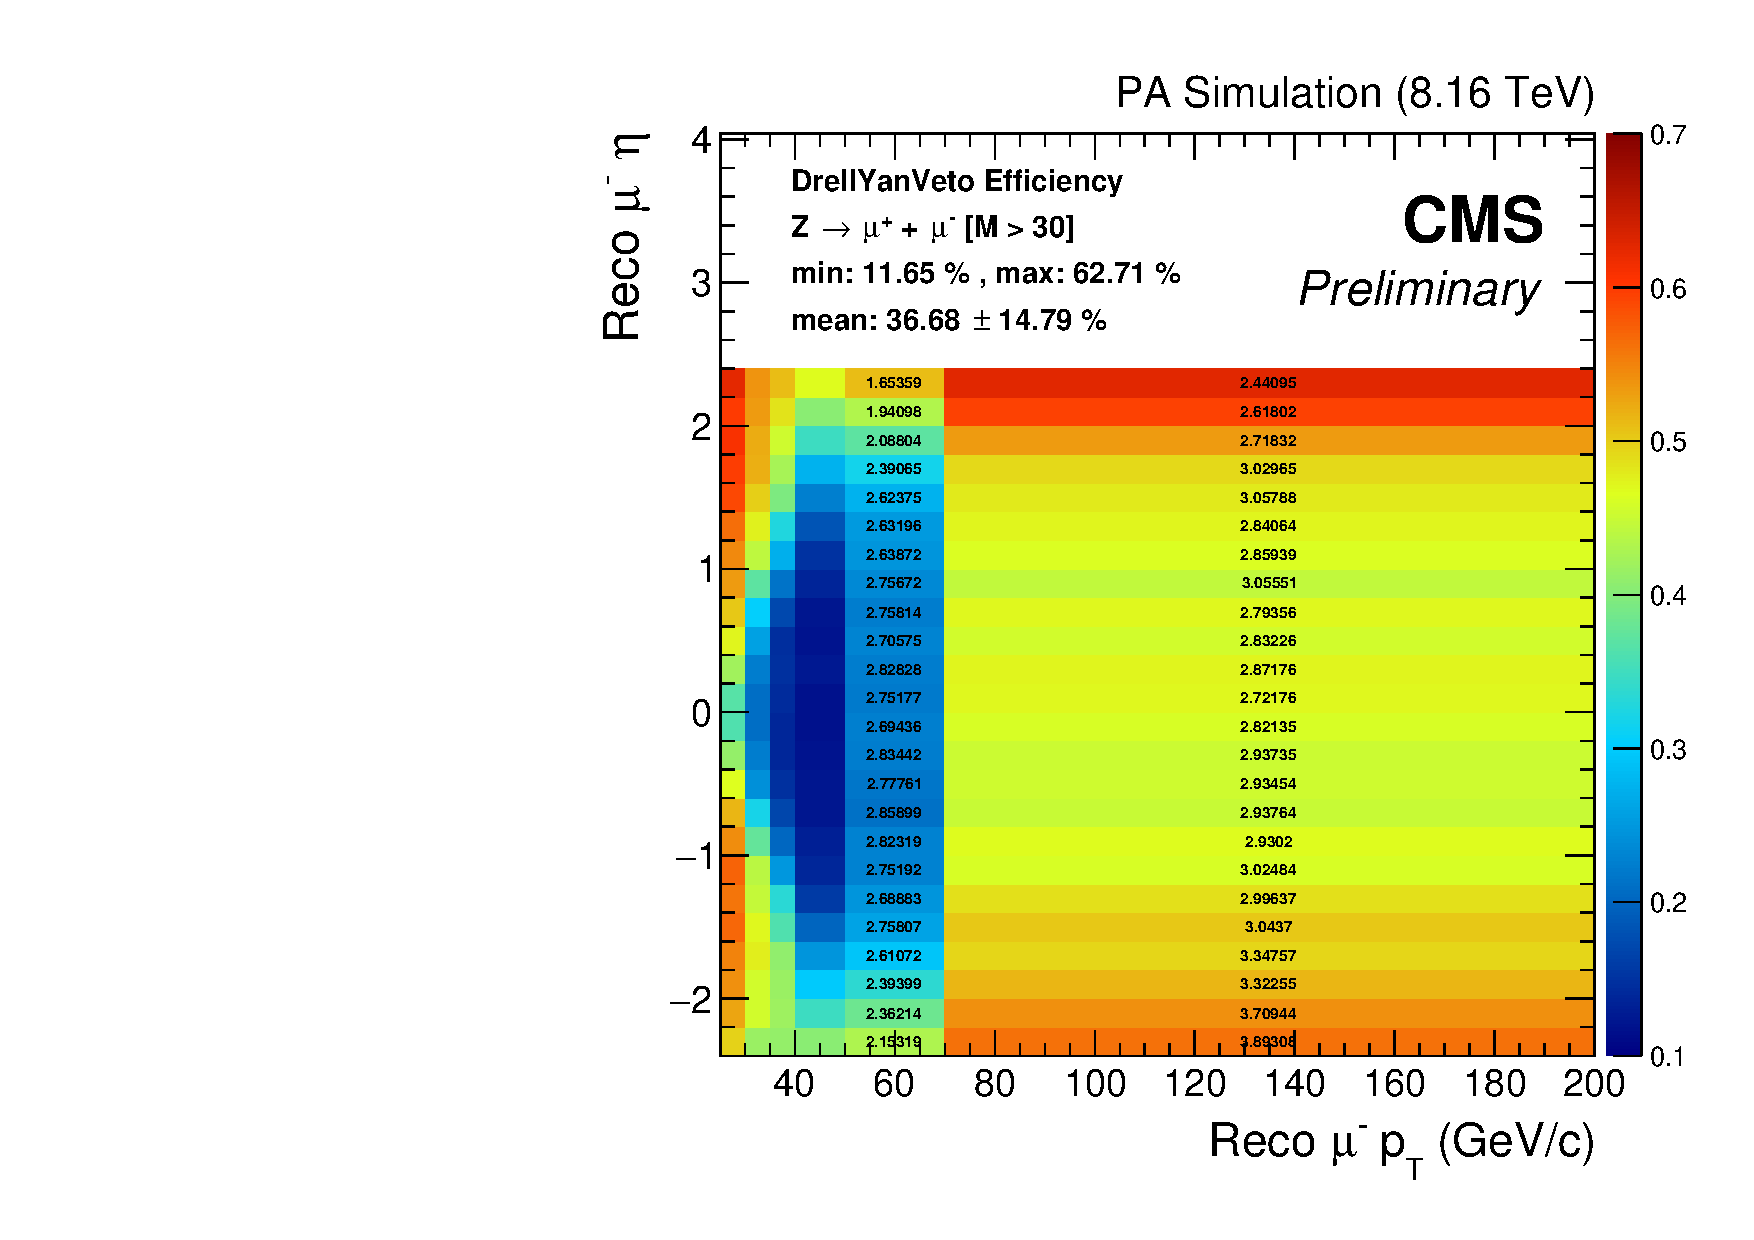
\includegraphics[width=0.45\textwidth]{Figures/WBoson/Analysis/Muon/Efficiency/Efficiency2D/Pt_Eta/MC_ZToMuMu_M_30_Inf/PA/pdf/eff2D_Pt_Eta_MC_ZToMuMu_M_30_Inf_PA_Minus_DrellYanVeto}
   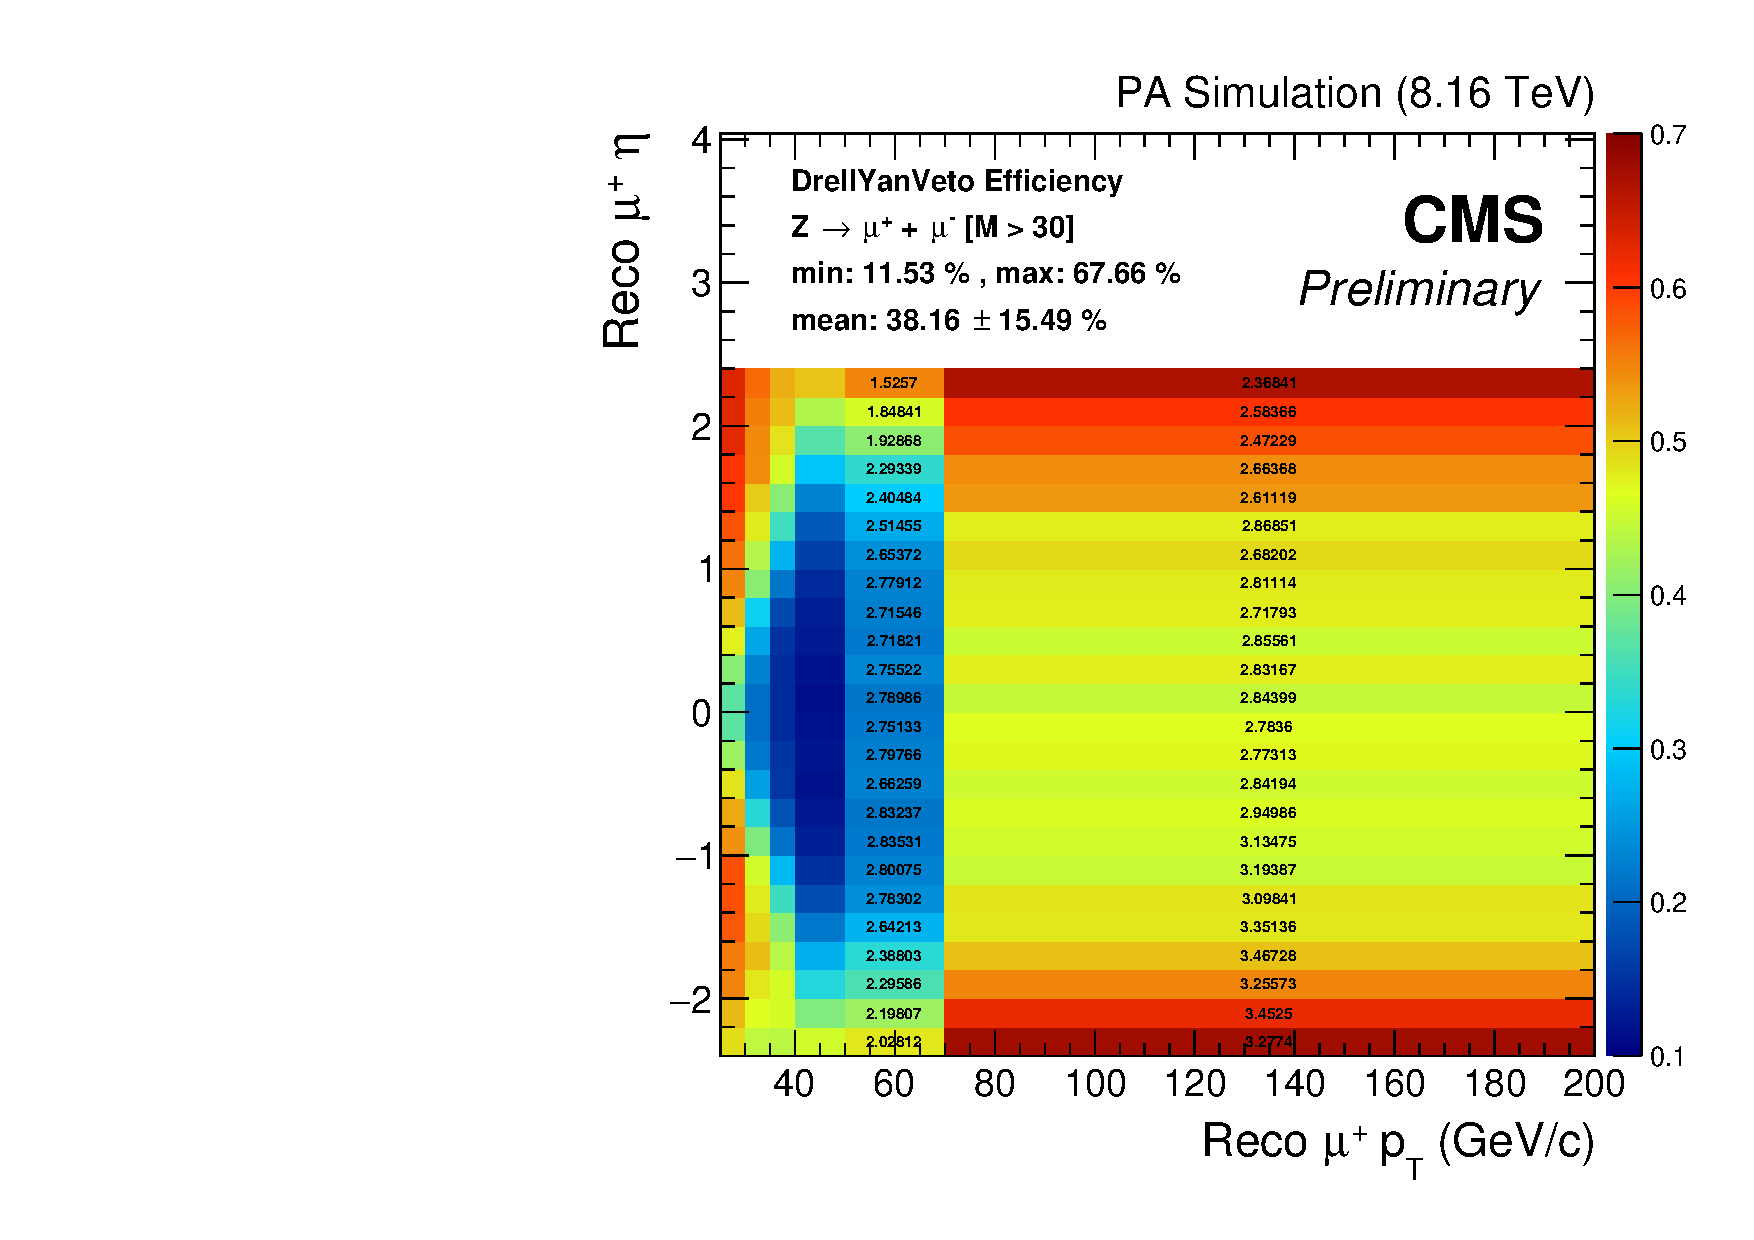
\includegraphics[width=0.45	\textwidth]{Figures/WBoson/Analysis/Muon/Efficiency/Efficiency2D/Pt_Eta/MC_ZToMuMu_M_30_Inf/PA/pdf/eff2D_Pt_Eta_MC_ZToMuMu_M_30_Inf_PA_Plus_DrellYanVeto}
   \caption{Survival probablity of single muons from Drell-Yan ($M > 30$~\GeVcc) MC sample  as a function of the reconstructed muon $\eta$ and \pt, separated in negative (left) and positive (right) charged muons. The \pPb and \Pbp MC samples are combined as described in \sect{sec:WBoson_Analysis_CombiningBeamDirection}. The relative statistical efficiency uncertainties scaled by 100 are shown for the two highest \pt bins. Reconstructed muons are required to be within $\pt > 25$~\GeVc and $|\eta| < 2.4$, be trigger matched and pass the Isolation and Tight ID selection criteria.}
   \label{fig:DrellYanVetoZEfficiency2D}
 \end{center}
\end{figure}


\subsubsection{Background Sources} \label{sec:WBoson_Analysis_BackgroundSources}

A high \pt muon constitute a signature common to a few processes which needs to be identified in order to estimate the \W signal events. The background processes can be classified as reducible and irreducible according to its characteristics.

The \emph{reducible} backgrounds constitute muon decays that can be clearly tagged and removed from the signal. This type of backgrounds represents the dominant sources:

\begin{itemize}
\item QCD multi-jets containing a high \pt muon (mostly from b-jets): This background is characterised by a low \ETslash and a large energy deposit surrounding the muon. A relative isolation cut around the muon is used to reduce this source.
\item \mumu pairs from Drell-Yan decays (\DY), or high-\pt resonances, having the two muons inside the acceptance window of this analysis. This background is vetoed from the analysis by removing events with two opposite sign muons as described in \sect{sec:WBoson_Analysis_DrellYanVeto}.
\end{itemize}

The \emph{irreducible} backgrounds represent muon decays that are impossible to prevent from interfering with the signal. This type of backgrounds are estimated by using MC templates or data-driven techniques. These sources include:

\begin{itemize}
\item \WToTauNu or \DYToTauTau events where the \PGt\ decays to a \PGm.
\item Top quark decays ($\PQt\to\W\PQb$) producing a \W plus a \PQb-jet.
\item \DY to muon decays where one muon is not identified or is produced outside of the acceptance window.
\item QCD multi-jets events that pass the muon isolation cut.
\end{itemize}


\subsubsection{\PW\ Boson Selection} \label{sec:WBoson_Analysis_WSelection}

The \W candidate selection consists of the detection of a high \pt muon, passing all identification criteria explained in \sect{sec:WBoson_Analysis_MuonIdentification}. In this analysis, the leading muon, as defined in \sect{sec:WBoson_Analysis_LeadingMuon}, is required to have a $\pt > 25$~\GeVc and be trigger matched (see \sect{sec:WBoson_Analysis_MuonTrigger}). The QCD background is reduced by applying the optimal muon isolation cut ($iso < 0.15$) defined in \sect{sec:WBoson_Analysis_MuonIsolation}. Since high \pt muons can also come from Drell-Yan or resonance decays, a dimuon veto is applied, as described in \sect{sec:WBoson_Analysis_DrellYanVeto}, to remove this potential source of background.

The other signature of a \W event is a high \pt neutrino, estimated through the \ETslash. No explicit cut is applied on \ETslash. The missing transverse energy is directly used to build templates and extract the yields by fitting the signal and background components.


\subsubsection{Summary of Event Selection}\label{sec:WBoson_Analysis_SignalEventSelection}

The conditions used in this analysis to define the signal and background regions of interest, are illustrated in \fig{fig:EventSelectionDiagram}.

\begin{figure}[htb]
 \begin{center}
   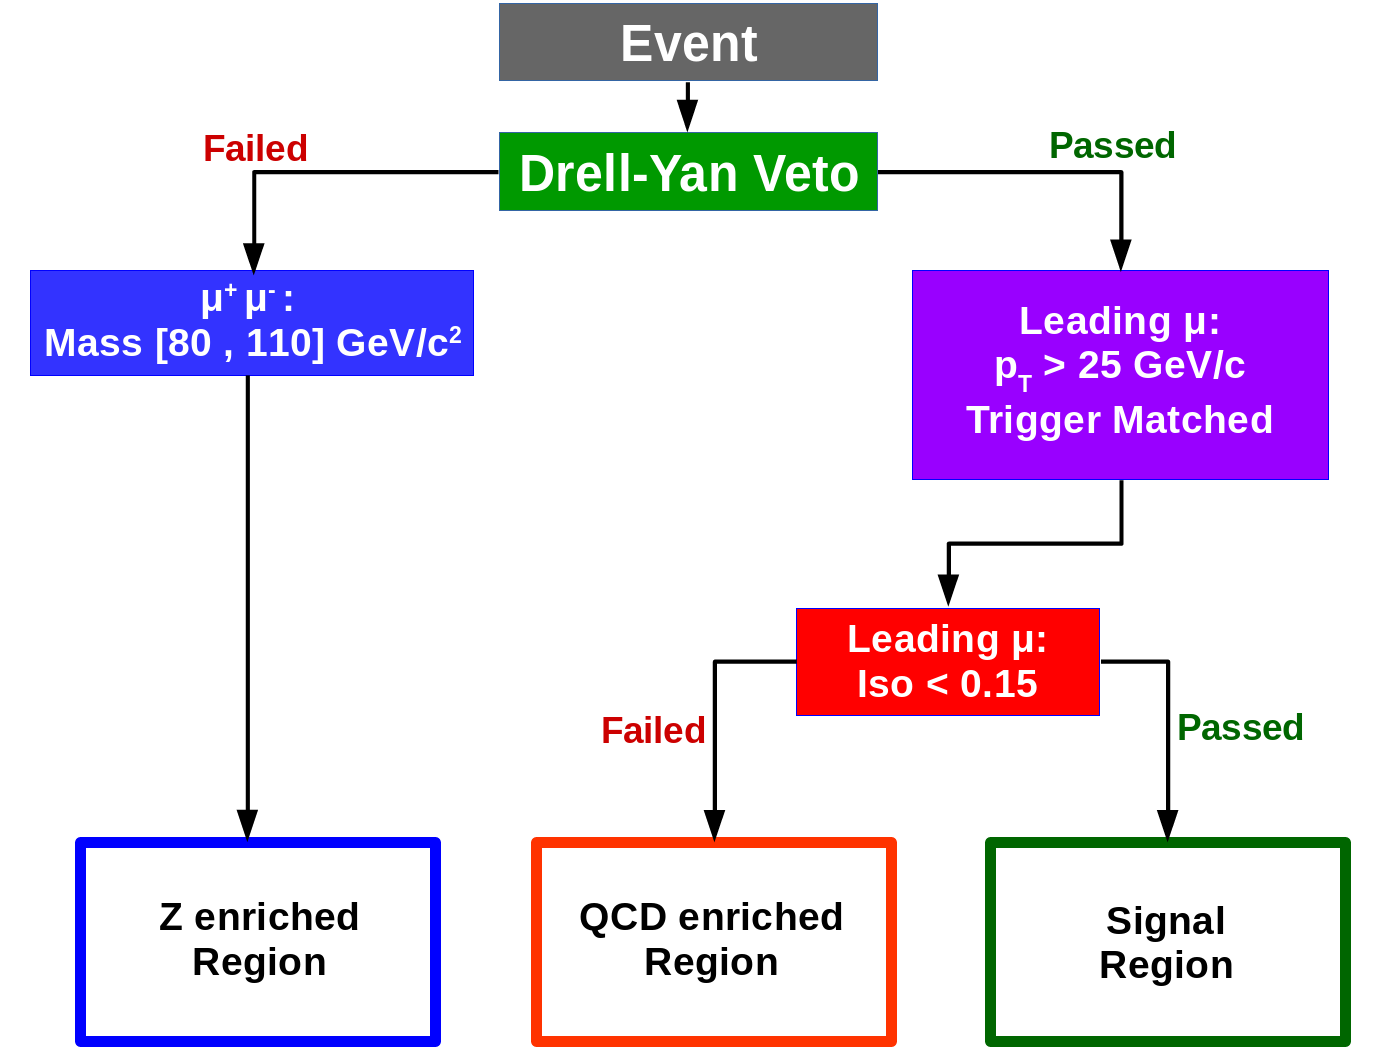
\includegraphics[width=0.9\textwidth]{Figures/WBoson/Analysis/EventSelection/FlowChar.png}
   \caption{Flowchart illustrating the way the events are classified}
   \label{fig:EventSelectionDiagram}
 \end{center}
\end{figure}


\subsubsection{Event Activity Reweighting}\label{sec:WBoson_Analysis_EventActivityReweighting}

The \pPb underlying event (UE) activity has been checked in a \DYToMuMu enriched sample of data and MC by comparing the distribution of the number of tracks and the energy deposited in the Hadron Forward (HF) calorimeters. The official MC samples embedded in \EPOS minimum bias events are not currently able to reproduce the UE present in \pPb data, as can be observed in \fig{fig:hfrew_1}. Since the muon isolation and the MET are computed by summing over particles, they are correlated with the UE and therefore, any disagreement in the modelling of the event activity can have an impact on the efficiency and the signal extraction. The disagreement between MC and data can be caused by several reasons:

\begin{enumerate}
 \item The presence of hard probes such as \Z or \W bosons bias the event activity towards higher multiplicity compared to minimum bias events.
 \item The generator does not model properly the soft part of the event.
 \item \GEANT4 does not simulate properly the detector responce of the soft particles from the UE.
 \item The MC samples do not contain pileup events
\end{enumerate}

Therefore, in an effort to try to correct the UE in MC, mainly the mismodelling due to the first effect listed above, the MC distribution of the energy deposited in both sides of the HF calorimeters is reweighted to match the data in the Z enriched region. As can be seen in \fig{fig:hfrew_1} and \fig{fig:hfrew_2}, the HF reweighting significantly improves the MC-data agreement in the distribution of the HF energy\footnote{The reason why the HF distribution is not exactly the same between MC and data after applying the HF reweighting is because the plots are made including all Drell-Yan events while the corrections were derived within the Z mass region}, the number of tracks, the muon isolation and the MET. More details on the HF reweighting studies can be found in the analysis note of the Drell-Yan measurement in \pPb at 8.16~\TeV \cite{DY_pPb}.

\begin{figure}
 \begin{center}
  \includegraphics[width=0.48\textwidth,page=28]{Figures/WBoson/Analysis/EventSelection/dataMC_Powheg_MomUnCor_norew}\hfill
  \includegraphics[width=0.48\textwidth,page=28]{Figures/WBoson/Analysis/EventSelection/dataMC_Powheg_MomUnCor_rewboth}
  
  \includegraphics[width=0.48\textwidth,page=32]{Figures/WBoson/Analysis/EventSelection/dataMC_Powheg_MomUnCor_norew}\hfill
  \includegraphics[width=0.48\textwidth,page=32]{Figures/WBoson/Analysis/EventSelection/dataMC_Powheg_MomUnCor_rewboth}
 \end{center}
\caption{Impact of the two-sided HF reweighting on the data-MC agreement of a few variables. Left column: without the reweighting applied, right column: with the reweighting applied.
First row: two-sided HF energy and second row: number of offline tracks. The $\chi^2$/ndf is also given, with its probability between parentheses,
as well as the p-value from a Kolmogorov-Smirnov test. These figures were taken from the Drell-Yan analysis in \pPb at 8.16~\TeV \cite{DY_pPb}}
\label{fig:hfrew_1}
\end{figure}

\begin{figure}
 \begin{center}  
  \includegraphics[width=0.48\textwidth,page=68]{Figures/WBoson/Analysis/EventSelection/dataMC_Powheg_MomUnCor_norew}\hfill
  \includegraphics[width=0.48\textwidth,page=68]{Figures/WBoson/Analysis/EventSelection/dataMC_Powheg_MomUnCor_rewboth}
  
  \includegraphics[width=0.48\textwidth,page=57]{Figures/WBoson/Analysis/EventSelection/dataMC_Powheg_MomUnCor_norew}\hfill
  \includegraphics[width=0.48\textwidth,page=57]{Figures/WBoson/Analysis/EventSelection/dataMC_Powheg_MomUnCor_rewboth}
 \end{center}
\caption{Impact of the two-sided HF reweighting on the data-MC agreement of a few variables. Left column: without the reweighting applied, right column: with the reweighting applied.
First row: relative PF isolation and second row: PF MET. The $\chi^2$/ndf is also given, with its probability between parentheses,
as well as the p-value from a Kolmogorov-Smirnov test. These figures were taken from the Drell-Yan analysis in \pPb at 8.16~\TeV \cite{DY_pPb}}
\label{fig:hfrew_2}
\end{figure}

% END OF SUBSECTION
\clearpage

